% questions.tex —— 1960 年·全国卷 · 题目内容片段（无答案）
% 由 tools/generate_projects.py 依来源总账自 1960/1960_数学真题_试题.md 生成，勿手改（改源 MD 后重跑）


\begin{gktip}
\textbf{题面说明}：原卷按“一（1）至（6）、二、三、四、五”编号，本文统一映射为第 1—10 题。第五题的两个小题原卷要求选作一题；图形按原卷页面重绘为 TikZ 矢量源。
\end{gktip}

\gkpart{一、小题}

\begin{question}
\gkti{1}（1）解方程
\[
\sqrt{2x^2-5}-\sqrt{5x-7}=0
\]
（限定在实数范围内）。

\end{question}
\begin{question}
\gkti{2}（2）有 5 组篮球队，每组 6 队。首先每组中各队进行单循环比赛（即每两队比赛一次），然后各组的冠军再进行单循环比赛。问先后共比赛多少次？

\end{question}
\begin{question}
\gkti{3}（3）求证：等比数列的各项的对数组成等差数列。（这里所说的等比数列的各项都是正数。）

\end{question}
\begin{question}
\gkti{4}（4）求使等式
\[
\sqrt{1-\sin^2\frac{x}{2}}=\cos\frac{x}{2}
\]
成立的 $x$ 值的范围。（$x$ 是 $0^\circ$ 到 $720^\circ$ 的角。）

\Needspace{0.4\textheight}
\end{question}
\begin{question}
\gkti{5}（5）如图，用钢珠测量机件上一个小孔的直径。所用钢珠的中心是 $O$，直径是 $12$ 毫米。将钢珠放在这个小孔上，测得钢珠上端 $D$ 到机件平面的距离 $CD$ 是 $9$ 毫米。求这个小孔的直径 $AB$ 的长。
\nopagebreak[4]
\begin{center}% 1960 年全国卷第 5 题：钢珠测量机件小孔直径。
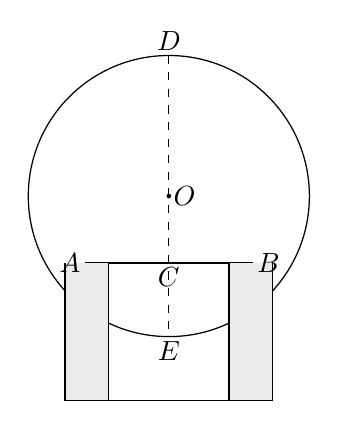
\begin{tikzpicture}[scale=0.85, line width=0.45pt,
  every node/.style={inner sep=1.5pt}]
  \coordinate (O) at (0,1.7);
  \coordinate (D) at (0,3.8);
  \coordinate (E) at (0,-0.4);
  \coordinate (C) at (0,0.7);
  \coordinate (A) at (-1.25,0.7);
  \coordinate (B) at (1.25,0.7);
  \draw (O) circle (2.1);
  \draw[dashed] (D)--(E);
  \draw (A)--(B);
  \draw[dashed] (A)--(C)--(B);
  \draw[fill=gray!15] (-1.55,0.7)--(-1.55,-1.35)--(-0.9,-1.35)--(-0.9,0.7);
  \draw[fill=gray!15] (0.9,0.7)--(0.9,-1.35)--(1.55,-1.35)--(1.55,0.7);
  \draw (-0.9,-1.35)--(0.9,-1.35);
  \fill (O) circle (0.035);
  \node[anchor=south] at (D) {$D$};
  \node[anchor=west] at (O) {$O$};
  \node[anchor=north] at (C) {$C$};
  \node[anchor=east] at (A) {$A$};
  \node[anchor=west] at (B) {$B$};
  \node[anchor=north] at (E) {$E$};
\end{tikzpicture}
\end{center}
\nopagebreak[4]
\Needspace{0.4\textheight}
\end{question}
\begin{question}
\gkti{6}（6）四棱锥 $P$—$ABCD$ 的底面是一个正方形。$PA$ 与底面垂直。已知 $PA$ 是 $3$ 厘米，$P$ 点到 $BC$ 的距离是 $5$ 厘米。求 $PC$ 的长。
\nopagebreak[4]
\begin{center}% 1960 年全国卷第 6 题：底面为正方形的四棱锥 P-ABCD。
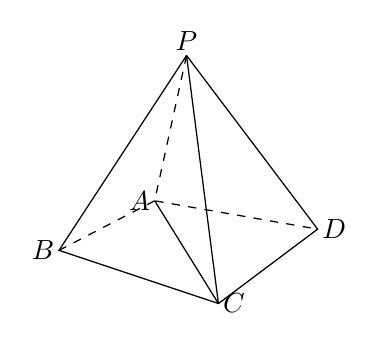
\begin{tikzpicture}[scale=0.9, line width=0.45pt,
  every node/.style={inner sep=1.5pt}]
  \coordinate (P) at (-0.2,2.7);
  \coordinate (A) at (-0.65,0.65);
  \coordinate (B) at (-2.0,-0.05);
  \coordinate (C) at (0.25,-0.8);
  \coordinate (D) at (1.65,0.25);
  \draw (P)--(B)--(C)--(D)--(P);
  \draw (P)--(C);
  \draw[dashed] (P)--(A)--(D);
  \draw[dashed] (A)--(B);
  \draw (A)--(C);
  \node[anchor=south] at (P) {$P$};
  \node[anchor=east] at (A) {$A$};
  \node[anchor=east] at (B) {$B$};
  \node[anchor=west] at (C) {$C$};
  \node[anchor=west] at (D) {$D$};
\end{tikzpicture}
\end{center}
\nopagebreak[4]
\end{question}
\gkpart{二、大题}

\begin{question}
\gkti{7}有一直圆柱，高是 $20$ 厘米，底面半径是 $5$ 厘米。它的一个内接长方体的体积是 $800$ 立方厘米。求这长方体的底面的长和宽。

\end{question}
\begin{question}
\gkti{8}从一船上看到在它的南 $30^\circ$ 东的海面上有一灯塔。船以 $30$ 里/小时的速度向正东南方向航行半小时后，看到这个灯塔在船的正西方。问这时船与灯塔的距离是多少？（精确到 $0.1$ 里。）

\end{question}
\begin{question}
\gkti{9}要在墙上开一矩形的大玻璃窗，周长限定为 $6$ 米。

（1）求以矩形的一条边长（$x$）表示窗户的面积（$y$）的函数式；

（2）求这函数图象的顶点的坐标、对称轴的方程；

（3）画出这函数的图象，并求出 $x$ 的允许值的范围。

\end{question}
\begin{question}
\gkti{10}下列（1）、（2）两题选作一题。

（1）已知方程
\[
2x^2-4x\sin\theta+3\cos\theta=0
\]
的两个根相等，且 $\theta$ 为锐角，求 $\theta$ 和这个方程的两个根。

（2）$a$ 是什么实数的时候，下列方程组的解是正数：
\[
\begin{cases}
2x+ay=4,\\
x+4y=8.
\end{cases}
\]

\end{question}